\documentclass{article}
\usepackage[OT1]{fontenc}
\usepackage[utf8]{inputenc}
\usepackage{amsthm,amssymb,amsmath}
\usepackage[a4paper, total={6.5in, 9in}]{geometry}
\usepackage[compact,explicit]{titlesec}
\usepackage[greek,english]{babel}
%\usepackage[iso-8859-7]{inputenc}
\usepackage[table]{xcolor}
%\usepackage{amsfonts}
%\usepackage{amsmath}
\usepackage{amssymb}
\usepackage{amsmath}
\usepackage{pgfplots}
\usepackage{tikz}
\usepackage{tikzscale}
\usepackage{array}
\usepackage{booktabs}
\usepackage{enumerate}
%\usepackage{color}
%AASFASFASF
\usepackage{empheq}
\usepackage{enumerate}
\usepackage{enumitem}
%\usepackage{gensymb}
\usepackage{graphicx}
\usepackage[space]{grffile}
\usepackage{ifthen}
%\usepackage{kerkis}
\usepackage{marginnote}
\usepackage{mathtools}
\usepackage{mdframed}
\usepackage{multirow}
%\usepackage{textgreek}
\usepackage{float}
\usepackage{slashbox}
\usepackage{listings}

\usepackage{caption}
\usepackage{afterpage}
\usepackage{forloop}
\usepackage{systeme}
\usepackage{cancel}
\usepackage{subcaption}
\usepackage{hyperref}
\usepackage{tikzsymbols}
\usetikzlibrary{calc}
\usepackage{changes}
\usepackage{cancel}
\setdeletedmarkup{\cancel{#1}}
%\usepackage{bbold}
%\newtheorem*{theorem}{Theorem}




\newcommand{\NN}{\mathbb{N}}
\newcommand{\ZZ}{\mathbb{Z}}
\newcommand{\RR}{\mathbb{R}}
\newcommand{\RRp}{\mathbb{R}^{+}}
\newcommand{\RRpp}{\mathbb{R}^{++}}
\newcommand{\QQ}{\mathbb{Q}}
\newcommand{\CC}{\mathbb{C}}
\newcolumntype{P}[1]{>{\centering\arraybackslash}p{#1}}

\newcommand{\tl}[1]{\textlatin{#1}}
\renewcommand\thesubfigure{(\roman{subfigure})}\usepackage{pgf, tikz}

\setlength{\arrayrulewidth}{1mm}
\setlength{\tabcolsep}{18pt}
\renewcommand{\arraystretch}{1.5}


\newcommand\blankpage{%
	\null
	\thispagestyle{empty}%
	\addtocounter{page}{-1}%
	\newpage}

\newcommand{\thewr}[1]{\mathrm{\ifthenelse{\equal{#1}{}}{}{#1,}\theta\epsilon\omega\rho}}
\newcommand{\peir}[1]{\mathrm{\ifthenelse{\equal{#1}{}}{}{#1,}\pi\epsilon\iota\rho}}
%\newcommand{\Upd}{\operatorname{U}^{\mathrm{M}}_{#1}}

\newlength\dlf
\newcommand\alignedbox[2]{
	% #1 = before alignment
	% #2 = after alignment
	&
	\begingroup
	\settowidth\dlf{$\displaystyle #1$}
	\addtolength\dlf{\fboxsep+\fboxrule}
	\hspace{-\dlf}
	\boxed{#1 #2}
	\endgroup
}

\setlist{  
	listparindent=\parindent%,
	%parsep=0pt
}

\hypersetup{
	colorlinks,
	linkcolor={red!50!black},
	citecolor={blue!50!black},
	urlcolor={blue!80!black}
}



%\let\thetitle\@title
%\let\theauthor\@author
%\let\thedate\@date

\DeclarePairedDelimiter\ceil{\lceil}{\rceil}

\DeclareMathOperator*{\argmax}{argmax} % thin space, limits underneath in display
\makeatother

\allowdisplaybreaks

%Η απόλυτη τιμή
\DeclarePairedDelimiter\abs{\lvert}{\rvert}


\renewcommand{\theenumi}{\roman{enumi}}


\begin{document}
	\greektext
	\captionsetup[figure]{labelfont={default},labelformat={default},labelsep=period,name={Σχήμα:}}
	\title{\tl{Assignment 1: Filtering and hybrid images}}						% Title
	\author{Μαυρογιώργης Δημήτρης, AM:2016030016\\Κολομβάκη Αφροδίτη, AM:2016030158\\Δελατόλας Θάνος, AM:2016030074}								% Author
	\date{\today}											% Date
	
	\makeatletter
	\let\thetitle\@title
	\let\theauthor\@author
	\let\thedate\@date
	\makeatother
	
	
	
	\begin{titlepage}
		\centering
		\vspace*{0.5 cm}
		\includegraphics[scale = 0.4]{polytexneio-logo.png}\\[1.0 cm]	% University Logo
		\textsc{\LARGE Μηχανικη Όραση }\\[2.0 cm]	
		\rule{\linewidth}{0.2 mm} \\[0.4 cm]
		{ \huge \bfseries \thetitle}\\
		\rule{\linewidth}{0.2 mm} \\[1.5 cm]
		
		\begin{minipage}{0.6\textwidth}
			
			\begin{flushright} \large
				\theauthor\\
				
			\end{flushright}
			
			\begin{flushright} \large
				\tl{\thedate}\\
				
			\end{flushright}
			
		\end{minipage}\\[2 cm]
		
	\end{titlepage}
	
	\newpage
	\section*{1. \tl{Introduction}}
	Οταν χρησιμοποιούμε \tl{low-pass} φίλτρα, όπως για παράδειγμα το \tl{Gaussian}, οι εικόνες που φιλτράρονται ειναι πιο \tl{smooth} ενω οταν χρησιμοποιούμε κάποιο \tl{high-pass} φιλτρο, η εικόνα που παίρνουμε ειναι πιο \tl{sharpened}.\\
	
	\noindent
	Μια \tl{hybrid} εικόνα δημιουργείται με το συνδιασμό μιας εικόνας που εχει υποστεί \tl{high-pass} φιλτραρισμα και μιας αλλης που εχει υποστεί \tl{low-pass} φιλτραρισμα. Το τελικό αποτέλεσμα το οποίο βλέπουμε είναι μια εικόνα της οποίας το περιεχόμενο αλλάζει ανάλογα με την απόσταση απο την οποία την κοιτάμε. Πιο συγκεκριμένα, οταν κοιτάμε την \tl{hybrid} εικόνα απο κάποια κοντινή απόσταση μπορούμε να διακρίνουμε την εικόνα που έχουμε περάσει απο το \tl{high-pass} φιλτρο ενω όταν βρισκόμαστε σε μεγαλύτερη απόσταση μπορούμε να δουμε την εικόνα που περάσαμε απο το \tl{low-pass} φιλτρο.\\
	
	\noindent
	Επιπλέον, αυτό που καθορίζει το πόσες υψηλές συχνότητες θα αποκόψουμε από την πρώτη εικόνα και πόσες χαμηλές συχνότητες θα παραμείνουν στη δεύτερη εικόνα καθορίζεται από μία ελεύθερη παράμετρο που ονομάζεται \tl{"cutoff-frequency"}.
	
	\section*{2. \tl{Implementation}}
	Αρχικά κληθήκαμε να υλοποιήσουμε μια \tl{custom imfilter} η οποία δέχεται μια εικόνα και ένα φίλτρο 
	και επίστρέφει την συνέλιξη των δυο. Όσον αφορά την υλοποίηση, αυτό που κάνουμε αρχικά είναι ένα 
	\tl{zero padding} περιμετρικά της εικόνας προκείμένου να μπορέσει να γίνει η συνέλιξη των εξωτερικών 
	pixel της με το φίλτρο. Πιο συγκεκριμένα, η συνάρτηση αποτελείται από ένα τριπλό \tl{nested-loop} μέσα στο 
	οποίο αθροίζουμε το γινόμενο κάθε \tl{pixel} της εικόνας με το φίλτρο. Αυτά τα τρία \tl{nested-loops}
	αντιστοιχούν στις τρεις διαστάσεις της εικόνας: χρωματικά κανάλια (\tl{RGB}), γραμμές και στήλες. Κατ' επέκταση,
	στην περίπτωση \tl{gray-scale} εικόνας το εξωτερικό \tl{loop} εκτελείται μόνο μια φορά με αποτέλεσμα να έχουμε
	ένα διπλό \tl{nested-loop}.\\
	
	\noindent
	Η σχέση που υλοποιεί η συνάρτηση είναι:
	\begin{align*}
		h[m,n] &= \sum_{k,l} g[k,l] \cdot f[m+k,n+l]
	\end{align*}
	\\\\
	\noindent
	Στη συνέχεια, για να ελέγξουμε τα αποτελέσματα της δικής μας υλοποίησης της \tl{imfilter}, εφαρμόσαμε σε μία εικόνα διάφορα φίλτρα, ενώ παράλληλα στο αρχείο \tl{assignment1\_filtering\_test.m} χρησιμοποιήσαμε τη συνάρτηση \tl{imfilter} της  \tl{Matlab} υπολογίζοντας και το \tl{MSE} μεταξύ των δύο εικόνων έτσι, ώστε να βεβαιωθούμε ότι τα αποτελέσματα που προκύπτουν είναι ακριβώς ίδια.
	\\\\
	\noindent
	Όσον αφορά τη δημιουργία της \tl{hybrid image}, δημιουργουμε ενα \tl{low-pass Gaussian} φίλτρο με την \tl{fspecial}, 
	το οποίο βαζουμε στη συνεχεια ως όρισμα μαζι με την εικόνα στη δική μας \tl{my\_imfilter}. Φιλτράρουμε, λοιπον, με τη 
	δικη μας \tl{my\_imfilter} την πρώτη εικόνα, για να εξαλείψουμε τα components που εχουν συχνότητες μεγαλύτερες απο το threshold, 
	διατηρώντας έτσι τις χαμηλές συχνότητες. Στη συνέχεια, εφαρμόζουμε το ίδιο φίλτρο στη δεύτερη εικόνα και αυτό που προκύπτει 
	το αφαιρούμε απο την original δεύτερη εικόνα, ωστε να «πετάξουμε» τις χαμηλες συχνότητες. Τέλος, συνδιάζουμε την εικόνα με 
	τις χαμηλές συχνότητες και την εικόναμε της υψηλές, ωστε να πάρουμε τη \tl{hybrid} εικόνα. 
	
	\pagebreak
	\section*{3. \tl{Results}}
	
	\begin{figure}[H]
		\centering
		\begin{subfigure}[t]{0.2\textwidth}
			\centering
			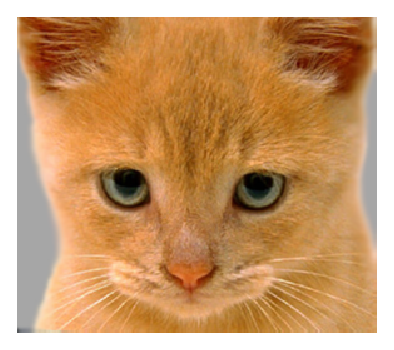
\includegraphics[height=4cm, width=\linewidth]{./res/fig_3_1.eps}
			\caption{\tl{Original Image}}
		\end{subfigure}%
		~
		\begin{subfigure}[t]{0.2\textwidth}
			\centering
			\includegraphics[height=4cm, width=\linewidth]{./res/fig_3_2.eps}
			\caption{\tl{Identity Filter}}
		\end{subfigure}%
		~
		\begin{subfigure}[t]{0.2\textwidth}
			\centering
			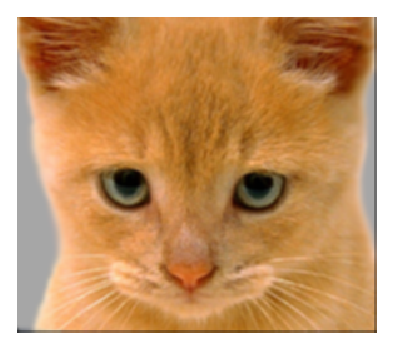
\includegraphics[height=4cm, width=\linewidth]{./res/fig_3_3.eps}
			\caption{\tl{Small Blur Filter}}
		\end{subfigure}	%
		~
		\begin{subfigure}[t]{0.2\textwidth}
			\centering
			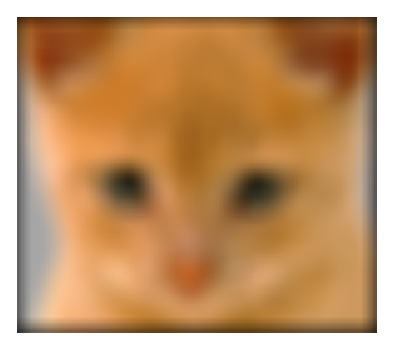
\includegraphics[height=4cm, width=\linewidth]{./res/fig_3_4.eps}
			\caption{\tl{Large Blur Filter}}
		\end{subfigure}
	
		\begin{subfigure}[t]{0.2\textwidth}
			\centering
			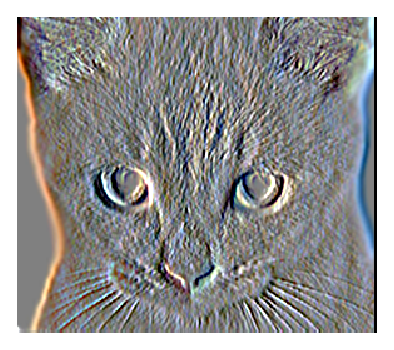
\includegraphics[height=4cm, width=\linewidth]{./res/fig_3_5.eps}
			\caption{\tl{Sobel Filter}}
		\end{subfigure}%
		~
		\begin{subfigure}[t]{0.2\textwidth}
			\centering
			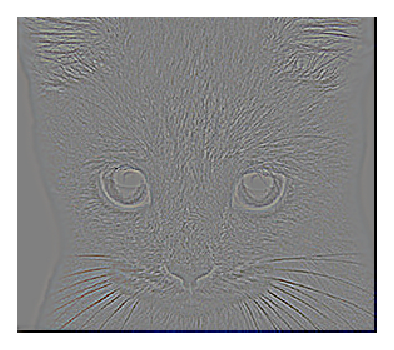
\includegraphics[height=4cm, width=\linewidth]{./res/fig_3_6.eps}
			\caption{\tl{Laplacian Filter}}
		\end{subfigure}%
		~
		\begin{subfigure}[t]{0.2\textwidth}
			\centering
			
\includegraphics[height=4cm, width=\linewidth]{./res/fig_3_7.eps}
			\caption{\tl{High Pass Filter}}
		\end{subfigure}
		\caption{Εφαρμογή μερικών βασικών φίλτρων στην αρχική εικόνα}
	\end{figure}

	\noindent
	Αρχικά, παρατηρούμε ότι από την εφαρμογή του \tl{identity filter} η εικόνα \tl{"ii"} είναι ακριβώς ίδια με την αρχική, επειδή το συγκεκριμένο φίλτρο έχει μονάδα στο κεντρικό \tl{pixel} και μηδενικά γύρω από αυτό, γεγονός που δεν επηρρεάζει την αρχική εικόνα.	Στην εικόνα \tl{"iii"} παρατηρούμε ότι μετά τη συνέλιξη με το φίλτρο γίνεται λίγο πιο θολή, ενώ στην εικόνα \tl{"iv"} βλέπουμε ότι γίνεται ακόμα πιο θολή, καθώς εφαρμόζουμε δύο φορές τη συνάρτηση \tl{my\_imfilter} με ένα Γκαουσιανό φίλτρο την πρώτη και το ανάστροφο του φίλτρου τη δεύτερη.\\
	
	\noindent
	Έπειτα, στην εικόνα \tl{"v"} παρατηρούμε ότι με την εφαρμογή του φίλτρου \tl{Sobel}, το οποίο βασίζεται στον υπολογισμό του \tl{gradient} της εικόνας, προκύπτουν τα \tl{edges} της εικόνας, δηλαδή παραμένουν κάποιες υψηλές συχνότητες της εικόνας. Tέλος, στις εικόνες \tl{"vi"} και \tl{"vii"}, όπου εφαρμόζουμε το \tl{Laplacian filter} και ένα \tl{high pass filter} αντίστοιχα, παρατηρούμε ότι έχουν παραμείνει και πάλι οι υψηλές συχνότητες.
	  
	\pagebreak
	\begin{figure}[H]
		\centering
		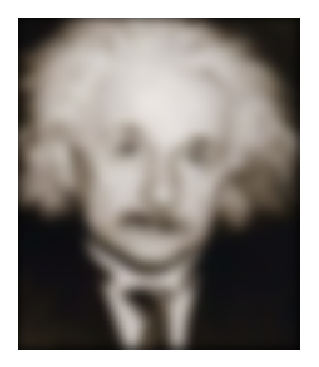
\includegraphics[scale=1]{./res/fig_1_1.eps}
		\caption{πρώτη εικόνα μετά απο την αφαίρεση των υψηλών συχνοτήτων επιλέγοντας \tl{Cutoff frequency}=5 (\tl{blurring})}
	\end{figure}
	
	\begin{figure}[H]
		\centering
		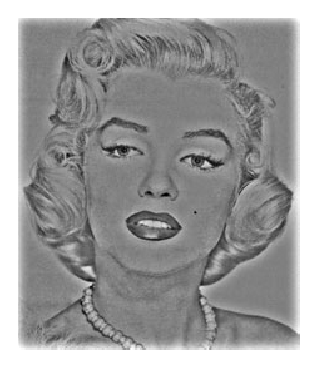
\includegraphics[scale=1]{./res/fig_1_2.eps}
		\caption{δεύτερη εικόνα ύστερα απο την αφαίρεση των χαμηλών συχνοτήτων με \tl{Cutoff frequency}=5}
	\end{figure}
	
 	\begin{figure}[H]
 		\centering
 		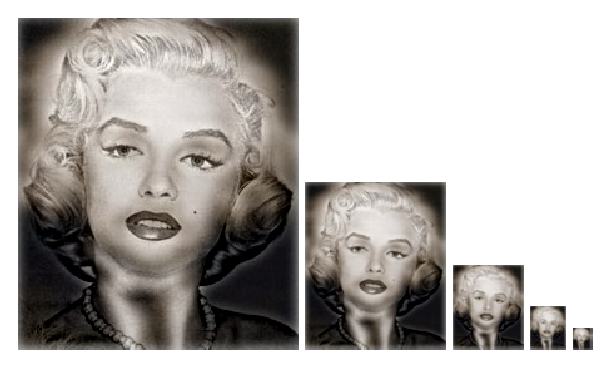
\includegraphics[scale=1]{./res/fig_1_3.eps}
 		\caption{\tl{hybrid image} με \tl{Cutoff frequency}=5}
 	\end{figure}
 
 	\begin{figure}[H]
 		\centering
 		
\includegraphics[scale=1]{./res/fig_2_1.eps}
 		\caption{πρώτη εικόνα μετά απο την αφαίρεση των υψηλών συχνοτήτων επιλέγοντας \tl{Cutoff frequency}=12}
 	\end{figure}
 	
 	\begin{figure}[H]
 		\centering
 		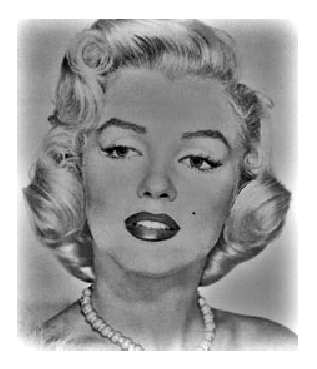
\includegraphics[scale=1]{./res/fig_2_2.eps}
 		\caption{δεύτερη εικόνα ύστερα απο την αφαίρεση των χαμηλών συχνοτήτων με \tl{Cutoff frequency}=12}
 	\end{figure}
 	
 	\begin{figure}[H]
 		\centering
 		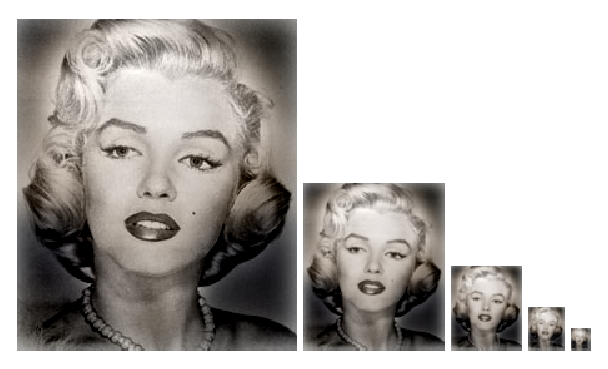
\includegraphics[scale=1]{./res/fig_2_3.eps}
 		\caption{\tl{hybrid image} με \tl{Cutoff frequency}=12}
 	\end{figure}
	
	\noindent
	Παρατηρώντας τα παραπάνω αποτελέσματα, βλέπουμε οτι όσο μεγαλύτερο είναι το \tl{cut-off frequency}, τόσο πιο πολύ χάνεται η εικόνα που έχει υποστεί \tl{low-pass filtering}, δηλαδη εκεινη που ειναι \tl{blurred}.\\
	
	\newpage
	\noindent
	Τώρα επαναλαμβάνουμε τη διαδικασία αλλά ως πρώτη εικόνα  επιλέγουμε τη \tl{marilyn} και ώς δεύτερη τον \tl{einstein}, οπότε η \tl{marilyn} θα φιλτραριστεί με το \tl{low-pass filter} ενω ο \tl{einstein} με το \tl{high-pass filter}. Τα αποτελέσματα είναι τα εξής:
	
	\begin{figure}[H]
		\centering
		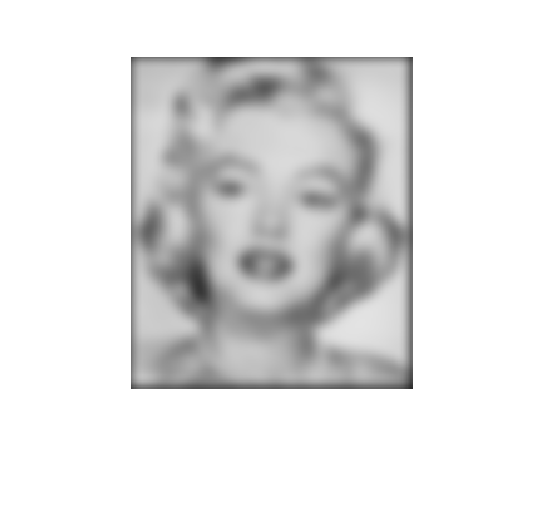
\includegraphics[scale=1]{./res/f1.eps}
		\caption{πρώτη εικόνα μετά απο την αφαίρεση των υψηλών συχνοτήτων επιλέγοντας \tl{Cutoff frequency}=5}
	\end{figure}
	
	\begin{figure}[H]
		\centering
		
\includegraphics[scale=1]{./res/f2.eps}
		\caption{δεύτερη εικόνα ύστερα απο την αφαίρεση των χαμηλών συχνοτήτων με \tl{Cutoff frequency}=5}
	\end{figure}
	
	\begin{figure}[H]
		\centering
		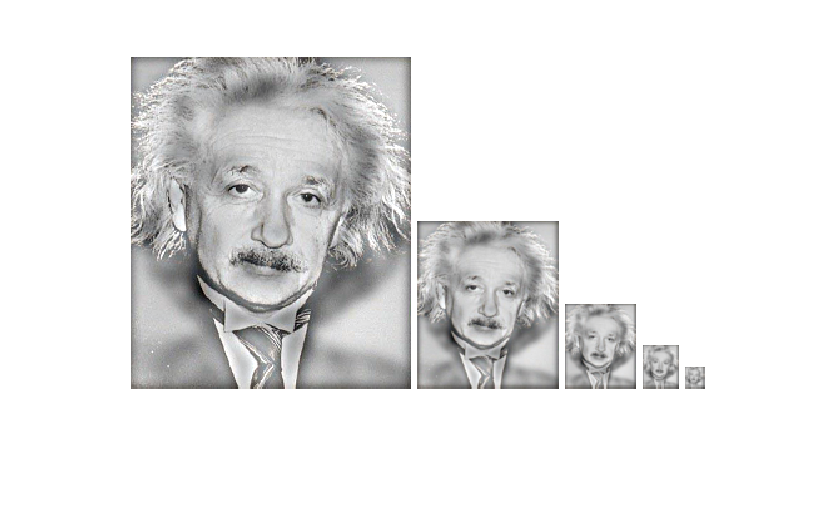
\includegraphics[scale=1]{./res/f3.eps}
		\caption{\tl{hybrid image} με \tl{Cutoff frequency}=5}
	\end{figure}
	\noindent
	Σε μερικές περιπτώσεις, έχει σημασία ποιά εικόνα θα επιλέξουμε να περάσουμε απο το \tl{high-pass filter} και ποια απο το \tl{low-pass filter}.Εδω παρατηρουμε οτι αν επιλέξουμε την εικόνα με το λιγότερο χρωμα, δηλαδη τη \tl{Marilyn} ως εκείνη που θα περάσουμε απο το \tl{low-pass filter}, το αποτέλεσμα ειναι καλύτερο από άποψη ομοιομορφίας χρωμάτων. Στο σχημα 4, το οποίο ειναι το αντίστοιχο, η μιση εικονα ειναι μαυρη και η αλλη μιση ασπρη, ενω στο σχημα 10 η κατανομη ειναι πιο ομοιομορφη. 
	\\
	\\
	\noindent
	\underline{Μερικά επιπλέον συμπεράσματα: }\\ \\
	\noindent
	Οι δυο εικόνες που συνδιάζουμε για να φτιάξουμε τη \tl{hybrid} δε μπορούν να είναι οποιεσδήποτε δυο εικόνες, αλλα θα πρεπει να ειναι \tl{aligned} και επισης τα χρώματα και η γεωμετρία τους να είναι τέτοια ωστε να δημιουργείται αυτη η ψευδαίσθηση που ψάχνουμε.\\ \\
	\noindent
	Τέλος, στα σχήματα 4,7 και 10 παρατηρούμε ότι στην πρωτη και πιο μεγαλη εικόνα βλέπουμε πιο έντονα την εικόνα που είχαμε περάσει από το \tl{high-pass} φίλτρο, ένω όσο πηγαινουμε προς τα δεξιά, δηλαδη οσο την κάνουμε \tl{downsample}, τόσο καλύτερα αρχίζει και φαίνεται η εικόνα με τη \tl{low-pass} πληροφορία. Πιο συγκεκριμένα, στο σχήμα 10, στην πιο μεγαλη εικονα (τερμα αριστερά) επικρατει η μορφή του \tl{Einstein} ενω όσο πηγαίνουμε προς τα δεξιά, στις μικρότερες εικόνες, επικρατει ολο και περισσότερο η μορφή της \tl{Marilyn}. 
\end{document}